\documentclass[10pt,a4paper]{article}

%% Language and font encodings
\usepackage[utf8]{inputenc}
\usepackage[english]{babel}
\usepackage[english]{isodate}
\usepackage[parfill]{parskip}


%% Sets page size and margins
\usepackage[a4paper,top=3cm,bottom=2cm,left=3cm,right=3cm,marginparwidth=1.75cm]{geometry}

%% Useful packages
\usepackage{amsmath}
\usepackage{graphicx}
\usepackage{float}
\usepackage{url}
\usepackage{listings}
\usepackage[colorinlistoftodos]{todonotes}
\usepackage[colorlinks=true, allcolors=blue]{hyperref}

\usepackage{authblk}

\lstdefinelanguage{F}{%
	language     = C,
	morekeywords = {fract},
	basicstyle=\ttfamily,
	keywordstyle=\color{blue}\ttfamily,
	stringstyle=\color{red}\ttfamily,
	commentstyle=\color{gray}\ttfamily,
	morecomment=[l][\color{magenta}]{\#}
}

\title{\textbf{FAC - User Manual}}
\author[1]{Mirko Bez}
\author[2]{Stefano Munari}
\affil[1]{\href{mailto:mirko.bez@studenti.unipd.it}{mirko.bez@studenti.unipd.it}}
\affil[2]{\href{mailto:stefano.munari.1@studenti.unipd.it}{stefano.munari.1@studenti.unipd.it}}

% Image directory
\graphicspath{{res/img/}}
% Set path for the sections
\makeatletter
\providecommand*{\input@path}{}
\g@addto@macro\input@path{{section/}}% append
\makeatother


\begin{document}
\maketitle
\tableofcontents
\listoffigures
\listoftables
\newpage
\section*{Introduction}

FAC is the front end part of a compiler which translates programs written in the
F language into a target representation. FAC is written in C using
flex \cite{flex-online} and bison \cite{bison-online}.
It is interesting to note that FAC can potentially support many target
representations.

\subsection*{Architecture}
Fig. \ref{fig:arch-ovw} describes the architecture of FAC.
Its high-level structure is formed by two macro components:
\begin{itemize}
\item Lexer - the lexical analyzer;
\item Parser - which is divided into three parts:
\begin{itemize}
	\item Syntax analysis;
	\item Static semantic analysis;
	\item Target code generation.
\end{itemize}
\end{itemize}

FAC has been written to be modular. Indeed, it is possible to translate any F
program into other representations simply by writing a new printer implementation.
\\
In FAC a printer is a component which takes the three address code (3AC) of an F
program given as input and generates a version of that code translated into a targeted
representation.
\\
Currently, FAC supports three printers:
\begin{itemize}
\item IR (Internal Representation) - useful for educational purposes or to quickly debug the 3AC;
\item C - prints a C program;
\item Java\footnote{for time reasons only the skeleton has been implemented} - prints a Java program.
\end{itemize}

We chose to use two different intermediate representations:
\begin{itemize}
\item Abstract Syntax Three (AST) - because it is easy to perform semantic analysis on this structure;
\item Three Address Code (3AC) - because it is easy to perform code generation by parsing this structure.
\end{itemize}

\begin{figure}[H]
  \centering
  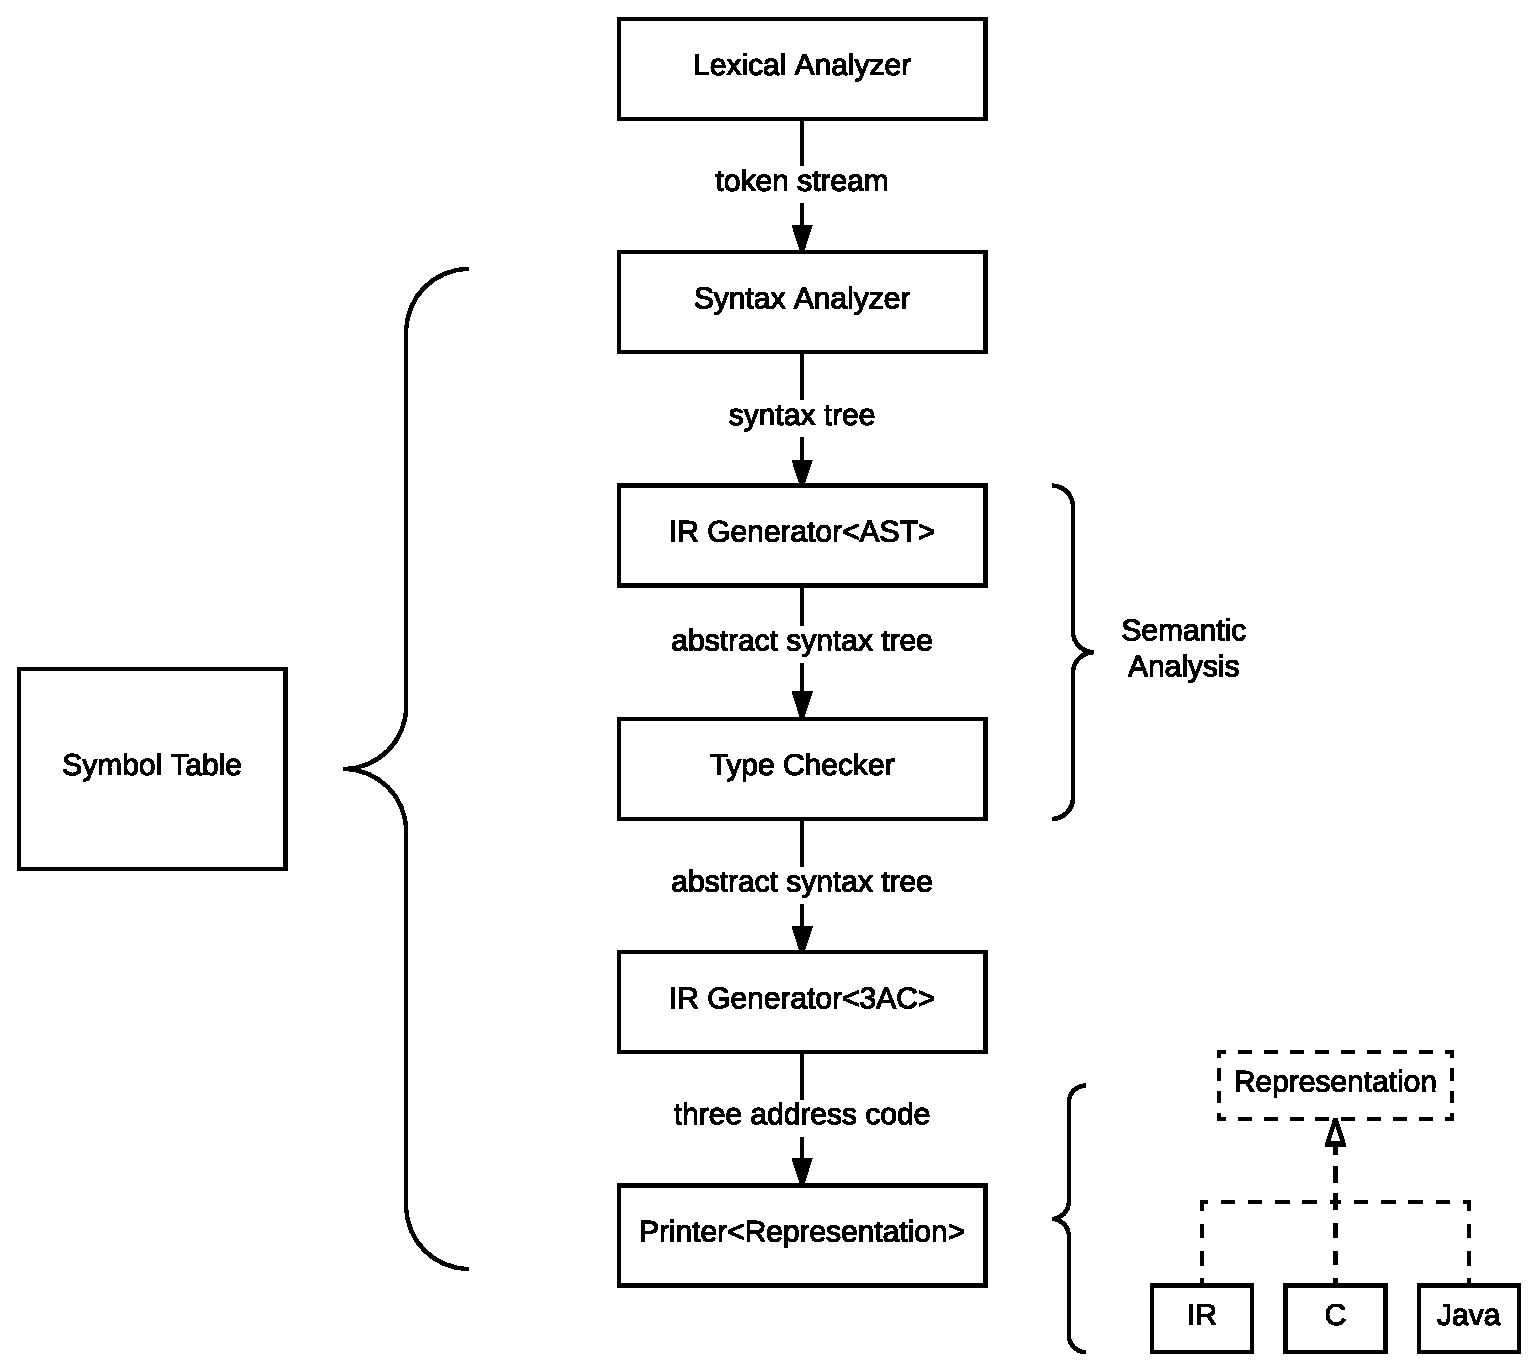
\includegraphics[width=.9\columnwidth]{img/eps/architecture.eps}
  \caption{Architectural Overview of the FAC compiler.}
  \label{fig:arch-ovw}
\end{figure}

%\input{compile}
%\input{run}
%\input{doc}
%\section{F Syntax}
The syntax is pretty similar to the C one except for the fract type that
is represented by writing \verb![numerator|denominator]!.
The operation that can be done on a value of type fract are described in Table
\ref{table:f:fract:operators} whereas the comparison on this type are reported
in Table \ref{table:f:fract:comparison:operators}.
The operators for the boolean type are listed in table 
\ref{table:f:bool:operators}.





%	&	\verb|+ -|	& Unary plus and minus & Right-to-left \\
%	& \verb|* /| & fract multiplication and division & Left-to-right \\ 
\begin{table}[h]
\centering
\begin{tabular}{|c|c|c|}
\hline
\textbf{Operator} & \textbf{Description} & \textbf{Associativity} \\ 
\hline
\verb|+ -| & Unary plus and minus 	& Right-to-left	\\
\verb|* /| & fract multiplication and division & Left-to-right \\ 
\verb|+ -| & fract sum and difference & Left-to-right \\
\hline
\end{tabular}
\label{table:f:fract:operators}
\caption{F operators that can be applied to fract values and return results
of the same type.}

\end{table}

\begin{table}[h]
\centering
\begin{tabular}{|c|c|c|}
\hline
\textbf{Operator} & \textbf{Description} & \textbf{Associativity} \\ 
\hline
\verb|<|	& less than	& Right-to-left	\\
\verb|<=|	& less than or equal to	& Left-to-right \\ 
\verb|==|	& equality & Left-to-right \\
\verb|<>|	& disequality & Left-to-right \\
\verb|>|	& bigger than & Left-to-right\\
\verb|>=|	& bigger than or equal to & Left-to-right \\
\hline
\end{tabular}
\caption{Fract comparison operators that return boolean values.}
\label{table:f:fract:comparison:operators}
\end{table}


\begin{table}[h]
\centering

\begin{tabular}{|c|l|l|l|l|}
\hline
\textbf{Operator} & \textbf{Description} & \textbf{Associativity} \\ 
\hline
\verb|!|	& Logial negation	& Right-to-left	\\
\verb|<->| & logical biimplication (boolean equality) & Left-to-right \\ \hline
\verb|XOR| & logical xor (boolean disequality) & Left-to-right \\ \hline
\verb|->|  & logical implication & Left-to-right \\ \hline
\verb!||!  & logical or & Left-to-right\\ \hline
\verb|&&|	& logical and & Left-to-right\\ \hline
\hline
\end{tabular}
\caption{F operation that can be applied on boolean operator}
\label{table:f:bool:operators}
\end{table}

\end{document}
